% Options for packages loaded elsewhere
\PassOptionsToPackage{unicode}{hyperref}
\PassOptionsToPackage{hyphens}{url}
\PassOptionsToPackage{dvipsnames,svgnames,x11names}{xcolor}
%
\documentclass[
  letterpaper,
  DIV=11,
  numbers=noendperiod]{scrartcl}

\usepackage{amsmath,amssymb}
\usepackage{iftex}
\ifPDFTeX
  \usepackage[T1]{fontenc}
  \usepackage[utf8]{inputenc}
  \usepackage{textcomp} % provide euro and other symbols
\else % if luatex or xetex
  \usepackage{unicode-math}
  \defaultfontfeatures{Scale=MatchLowercase}
  \defaultfontfeatures[\rmfamily]{Ligatures=TeX,Scale=1}
\fi
\usepackage{lmodern}
\ifPDFTeX\else  
    % xetex/luatex font selection
\fi
% Use upquote if available, for straight quotes in verbatim environments
\IfFileExists{upquote.sty}{\usepackage{upquote}}{}
\IfFileExists{microtype.sty}{% use microtype if available
  \usepackage[]{microtype}
  \UseMicrotypeSet[protrusion]{basicmath} % disable protrusion for tt fonts
}{}
\makeatletter
\@ifundefined{KOMAClassName}{% if non-KOMA class
  \IfFileExists{parskip.sty}{%
    \usepackage{parskip}
  }{% else
    \setlength{\parindent}{0pt}
    \setlength{\parskip}{6pt plus 2pt minus 1pt}}
}{% if KOMA class
  \KOMAoptions{parskip=half}}
\makeatother
\usepackage{xcolor}
\setlength{\emergencystretch}{3em} % prevent overfull lines
\setcounter{secnumdepth}{-\maxdimen} % remove section numbering
% Make \paragraph and \subparagraph free-standing
\makeatletter
\ifx\paragraph\undefined\else
  \let\oldparagraph\paragraph
  \renewcommand{\paragraph}{
    \@ifstar
      \xxxParagraphStar
      \xxxParagraphNoStar
  }
  \newcommand{\xxxParagraphStar}[1]{\oldparagraph*{#1}\mbox{}}
  \newcommand{\xxxParagraphNoStar}[1]{\oldparagraph{#1}\mbox{}}
\fi
\ifx\subparagraph\undefined\else
  \let\oldsubparagraph\subparagraph
  \renewcommand{\subparagraph}{
    \@ifstar
      \xxxSubParagraphStar
      \xxxSubParagraphNoStar
  }
  \newcommand{\xxxSubParagraphStar}[1]{\oldsubparagraph*{#1}\mbox{}}
  \newcommand{\xxxSubParagraphNoStar}[1]{\oldsubparagraph{#1}\mbox{}}
\fi
\makeatother


\providecommand{\tightlist}{%
  \setlength{\itemsep}{0pt}\setlength{\parskip}{0pt}}\usepackage{longtable,booktabs,array}
\usepackage{calc} % for calculating minipage widths
% Correct order of tables after \paragraph or \subparagraph
\usepackage{etoolbox}
\makeatletter
\patchcmd\longtable{\par}{\if@noskipsec\mbox{}\fi\par}{}{}
\makeatother
% Allow footnotes in longtable head/foot
\IfFileExists{footnotehyper.sty}{\usepackage{footnotehyper}}{\usepackage{footnote}}
\makesavenoteenv{longtable}
\usepackage{graphicx}
\makeatletter
\newsavebox\pandoc@box
\newcommand*\pandocbounded[1]{% scales image to fit in text height/width
  \sbox\pandoc@box{#1}%
  \Gscale@div\@tempa{\textheight}{\dimexpr\ht\pandoc@box+\dp\pandoc@box\relax}%
  \Gscale@div\@tempb{\linewidth}{\wd\pandoc@box}%
  \ifdim\@tempb\p@<\@tempa\p@\let\@tempa\@tempb\fi% select the smaller of both
  \ifdim\@tempa\p@<\p@\scalebox{\@tempa}{\usebox\pandoc@box}%
  \else\usebox{\pandoc@box}%
  \fi%
}
% Set default figure placement to htbp
\def\fps@figure{htbp}
\makeatother

\usepackage{booktabs}
\usepackage{longtable}
\usepackage{array}
\usepackage{multirow}
\usepackage{wrapfig}
\usepackage{float}
\usepackage{colortbl}
\usepackage{pdflscape}
\usepackage{tabu}
\usepackage{threeparttable}
\usepackage{threeparttablex}
\usepackage[normalem]{ulem}
\usepackage{makecell}
\usepackage{xcolor}
\usepackage{siunitx}

    \newcolumntype{d}{S[
      table-align-text-before=false,
      table-align-text-after=false,
      input-symbols={-,\*+()}
    ]}
  
\KOMAoption{captions}{tableheading}
\makeatletter
\@ifpackageloaded{caption}{}{\usepackage{caption}}
\AtBeginDocument{%
\ifdefined\contentsname
  \renewcommand*\contentsname{Table of contents}
\else
  \newcommand\contentsname{Table of contents}
\fi
\ifdefined\listfigurename
  \renewcommand*\listfigurename{List of Figures}
\else
  \newcommand\listfigurename{List of Figures}
\fi
\ifdefined\listtablename
  \renewcommand*\listtablename{List of Tables}
\else
  \newcommand\listtablename{List of Tables}
\fi
\ifdefined\figurename
  \renewcommand*\figurename{Figure}
\else
  \newcommand\figurename{Figure}
\fi
\ifdefined\tablename
  \renewcommand*\tablename{Table}
\else
  \newcommand\tablename{Table}
\fi
}
\@ifpackageloaded{float}{}{\usepackage{float}}
\floatstyle{ruled}
\@ifundefined{c@chapter}{\newfloat{codelisting}{h}{lop}}{\newfloat{codelisting}{h}{lop}[chapter]}
\floatname{codelisting}{Listing}
\newcommand*\listoflistings{\listof{codelisting}{List of Listings}}
\makeatother
\makeatletter
\makeatother
\makeatletter
\@ifpackageloaded{caption}{}{\usepackage{caption}}
\@ifpackageloaded{subcaption}{}{\usepackage{subcaption}}
\makeatother

\usepackage{bookmark}

\IfFileExists{xurl.sty}{\usepackage{xurl}}{} % add URL line breaks if available
\urlstyle{same} % disable monospaced font for URLs
\hypersetup{
  pdftitle={Primary data exploration},
  pdfauthor={Stepan Polikanov},
  colorlinks=true,
  linkcolor={blue},
  filecolor={Maroon},
  citecolor={Blue},
  urlcolor={Blue},
  pdfcreator={LaTeX via pandoc}}


\title{Primary data exploration}
\usepackage{etoolbox}
\makeatletter
\providecommand{\subtitle}[1]{% add subtitle to \maketitle
  \apptocmd{\@title}{\par {\large #1 \par}}{}{}
}
\makeatother
\subtitle{Peasant unrest and imperial repression}
\author{Stepan Polikanov}
\date{}

\begin{document}
\maketitle


\pandocbounded{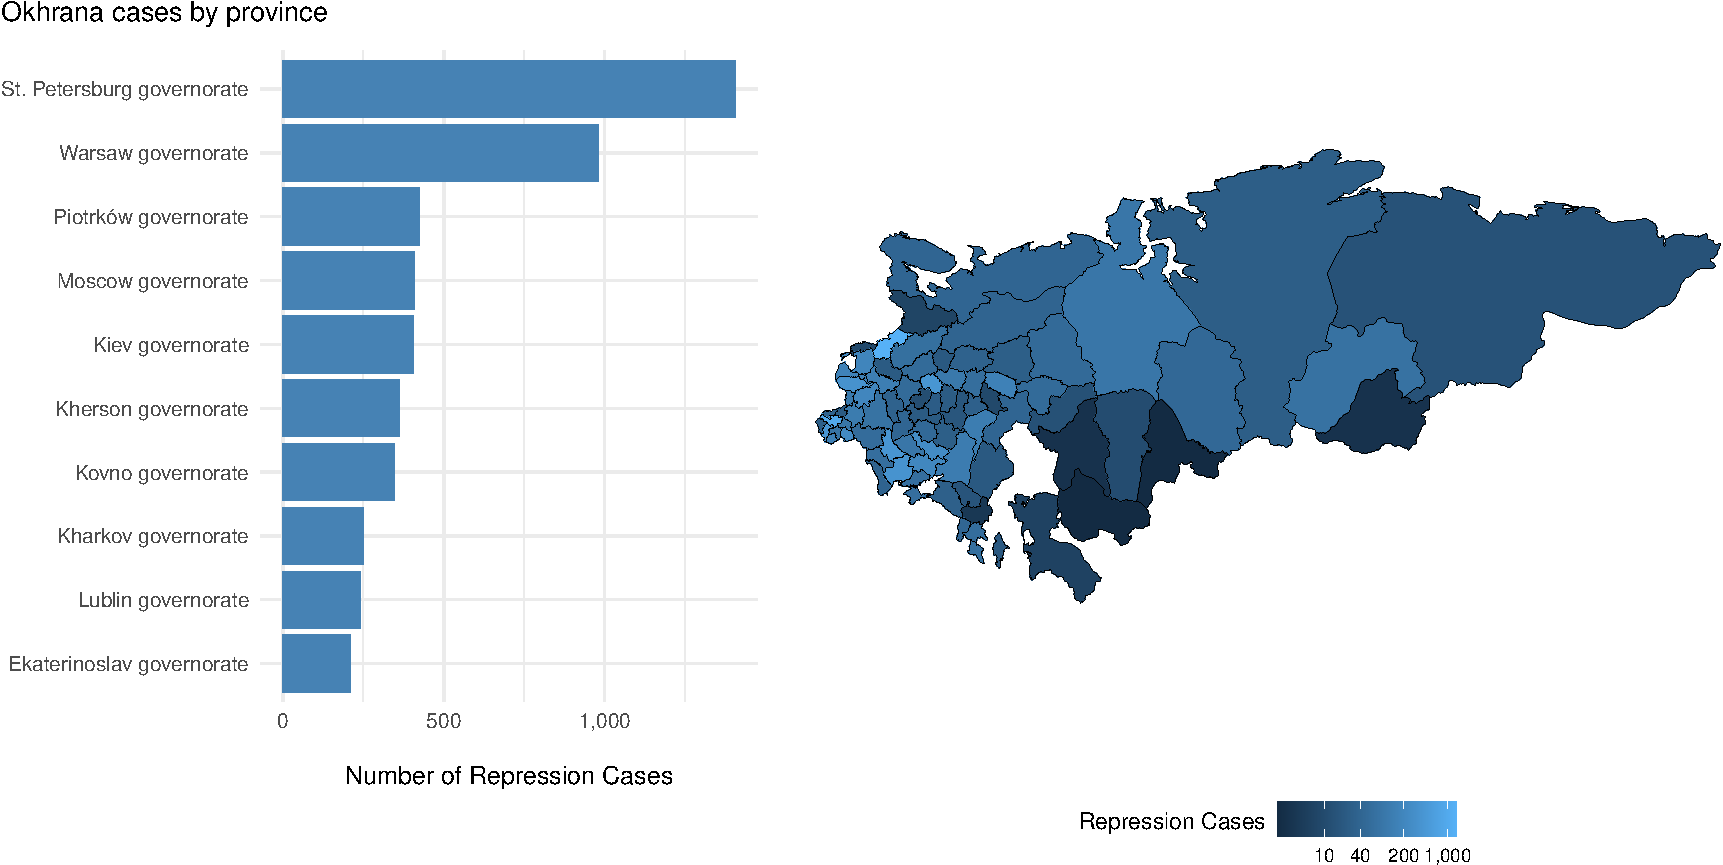
\includegraphics[keepaspectratio]{data_exploration_files/figure-pdf/descriptives-1.pdf}}

\begin{table}
\centering\centering
\resizebox{\ifdim\width>\linewidth\linewidth\else\width\fi}{!}{
\begin{tabular}[t]{lccccc}
\toprule
  & 1. Unrest only & 2. + Inequality & 3. + Serfdom \& Peasants & 4. + Urban \& Industrial & 5. + Urban × Inequality\\
\midrule
Intercept & \num{2.888}*** & \num{3.104}** & \num{3.190} & \num{2.403} & \num{0.939}\\
 & (\num{0.794}) & (\num{1.113}) & (\num{2.026}) & (\num{1.596}) & (\num{1.896})\\
(Log) Pre-1905 unrest & \num{0.302} & \num{0.485}+ & \num{0.352} & \num{0.534}+ & \num{0.548}*\\
 & (\num{0.194}) & (\num{0.255}) & (\num{0.339}) & (\num{0.268}) & (\num{0.265})\\
Land inequality (Gini) &  & \num{-1.241} & \num{-1.021} & \num{-1.561} & \num{0.112}\\
 &  & (\num{1.387}) & (\num{1.998}) & (\num{1.539}) & (\num{1.938})\\
Share of serfs (1858) &  &  & \num{0.543} & \num{0.060} & \num{0.279}\\
 &  &  & (\num{0.875}) & (\num{0.687}) & (\num{0.697})\\
Peasant land share &  &  & \num{0.210} & \num{-0.234} & \num{-0.625}\\
 &  &  & (\num{1.428}) & (\num{1.110}) & (\num{1.133})\\
Urbanization (1904) &  &  &  & \num{6.297}** & \num{23.888}+\\
 &  &  &  & (\num{1.826}) & (\num{12.758})\\
Manufacturing share (1904) &  &  &  & \num{0.385} & \num{-1.325}\\
 &  &  &  & (\num{3.804}) & (\num{3.957})\\
Urbanization × Inequality &  &  &  &  & \num{-19.778}\\
 &  &  &  &  & (\num{14.200})\\
\midrule
Num.Obs. & \num{52} & \num{49} & \num{49} & \num{48} & \num{48}\\
R2 & \num{0.046} & \num{0.073} & \num{0.081} & \num{0.458} & \num{0.483}\\
RMSE & \num{1.07} & \num{1.08} & \num{1.08} & \num{0.81} & \num{0.79}\\
\bottomrule
\multicolumn{6}{l}{\rule{0pt}{1em}+ p $<$ 0.1, * p $<$ 0.05, ** p $<$ 0.01, *** p $<$ 0.001}\\
\end{tabular}}
\end{table}

\pandocbounded{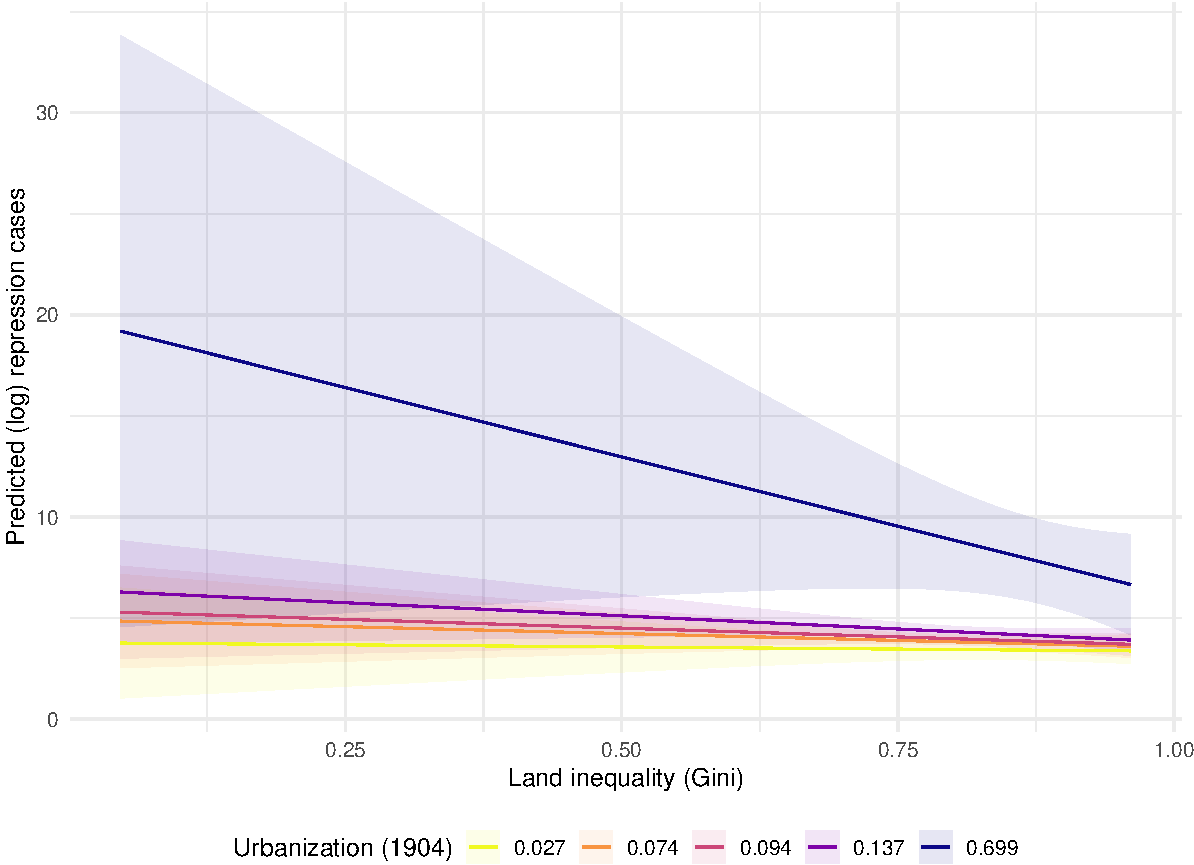
\includegraphics[keepaspectratio]{data_exploration_files/figure-pdf/plot the interaction-1.pdf}}

\begin{table}
\centering\centering
\resizebox{\ifdim\width>\linewidth\linewidth\else\width\fi}{!}{
\begin{tabular}[t]{lcccc}
\toprule
  & Control for population & Revolutionaries only & Alternative inequality measure & Negative Binomial\\
\midrule
Intercept & \num{-9.718}* & \num{2.241} & \num{1.208} & \num{31.326}*\\
 & (\num{3.881}) & (\num{1.557}) & (\num{1.076}) & (\num{43.501})\\
(Log) Pre-1905 unrest & \num{0.154} & \num{0.661}* & \num{0.465}+ & \num{1.799}*\\
 & (\num{0.265}) & (\num{0.262}) & (\num{0.260}) & (\num{0.420})\\
Land inequality (Gini) & \num{-1.877} & \num{-2.277} &  & \num{0.082}+\\
 & (\num{1.379}) & (\num{1.502}) &  & (\num{0.109})\\
Share of serfs (1858) & \num{0.302} & \num{-0.289} & \num{0.110} & \num{1.012}\\
 & (\num{0.619}) & (\num{0.670}) & (\num{0.686}) & (\num{0.604})\\
Peasant land share & \num{0.501} & \num{-0.601} & \num{0.553} & \num{0.475}\\
 & (\num{1.017}) & (\num{1.084}) & (\num{0.794}) & (\num{0.459})\\
Urbanization (1904) & \num{5.653}** & \num{4.182}* & \num{6.286}** & \num{593.362}***\\
 & (\num{1.644}) & (\num{1.782}) & (\num{1.827}) & (\num{934.820})\\
Manufacturing share (1904) & \num{1.221} & \num{2.336} & \num{0.216} & \num{0.709}\\
 & (\num{3.411}) & (\num{3.712}) & (\num{3.802}) & (\num{2.331})\\
\midrule
Num.Obs. & \num{48} & \num{48} & \num{48} & \num{48}\\
R2 & \num{0.577} & \num{0.390} & \num{0.445} & \\
R2 Adj. & \num{0.503} & \num{0.301} & \num{0.378} & \\
AIC & \num{520.2} & \num{472.8} & \num{529.4} & \num{531.2}\\
BIC & \num{537.1} & \num{487.8} & \num{542.4} & \num{546.2}\\
Log.Lik. & \num{-51.947} & \num{-56.729} & \num{-58.502} & \num{-257.593}\\
F & \num{7.806} & \num{4.377} & \num{6.725} & \num{7.637}\\
RMSE & \num{0.71} & \num{0.79} & \num{0.82} & \num{183.58}\\
\bottomrule
\multicolumn{5}{l}{\rule{0pt}{1em}+ p $<$ 0.1, * p $<$ 0.05, ** p $<$ 0.01, *** p $<$ 0.001}\\
\end{tabular}}
\end{table}




\end{document}
